\section{Experimental Analysis Results and Discussions}
\label{sec:results-and-discussions}

In this section, methodology presented in this study is applied on several data sets and results are presented. Firstly, evaluation metrics are defined for each stage of methodology to assess the performance of approach. Following this, methodology is applied on two data sets and results are explained with discussions.

Approach in this study is an aggregation of various methods and they are significantly different from each other in their mathematical background. Therefore, instead of a global evaluation metric for the complete methodology, each stage is evaluated within its evaluation metrics. In \textit{process model mining}, performance of process mining stage is measured by \textit{fitness} and \textit{appropriateness} which are defined in \cite{rozinat2008conformance}. In \textit{performance indicator analysis}, \textit{alignment costs} \cite{van2012replaying} are compared with process model mining metrics for replay phase. In clustering phase, \textit{within-SSE} analysis is undertaken to decide on the number of clusters. For \textit{mismatch pattern analysis}, number of mismatch patterns found are compared with the \textit{graph-edit similarity} \cite{dijkman2011similarity} of process models. In \textit{recommendation generation}, different threshold values are tried to check how many mismatch patterns are generated for organizations and how they could be used for focused analysis.

\subsection{Loan Application Process}
\label{subsec:loan-app-process}

In \textit{Loan Application Process} dataset there are a total of 475 cases and 2440 events with a fairly even distribution between variants and these variants are used as organizational logs and the methodology presented in this thesis study is be applied.

\begin{itemize}
  \item In \textit{Process Model Mining} stage, process models resulted with perfect fitness and high appropriateness as it is expected from a synthetically generated dataset without noise.
  \item In \textit{Performance Indicator Analysis} stage, firstly event logs are replayed over process models and performance indicators are calculated and then organizations are clustered based on their performance indicators. In order to avoid overfitting,  with two clusters, Variant \#1, \#2, and \#4 are grouped into one cluster where only Variant \#3 is left to other cluster. 
  \item In \textit{Mismatch Pattern Analysis} stage, number of mismatch patterns are analyzed with the \textit{graph-edit similarity} between each two organization. As the similarity between process models decreases our method spots more mismatch patterns for most of the variants and it ensures that the developed mismatch pattern analyzers work as expected for this dataset. 
  \item In \textit{Recommendation Generation} stage, an organization and performance difference threshold is selected as analysis input. For the selected organization's cluster, all other clusters are checked for performing better than the specified threshold. Instead of all mismatch patterns between organizations, only the mismatch patterns that are potential causes of other organizations to perform better are listed. For different threshold values, number of performance indicators that are performing better for the selected organization and spotted mismatch patterns are plotted in Figure~\ref{fig:loan-recommendation-generation-analysis}. 
    \begin{figure}
    	\centering
    	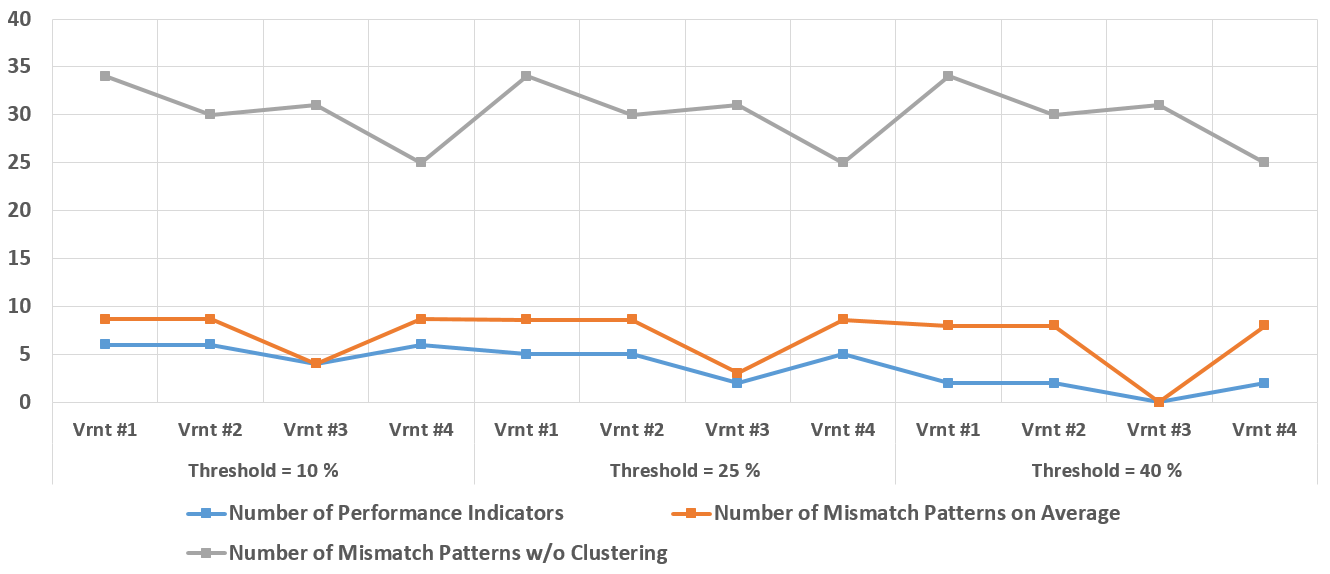
\includegraphics[width=\textwidth]{5_results_discussions/loan-application-process/recommendation-generation-analysis}
    	\caption{Recommendation Generation analysis for Loan Application Process dataset}
      \label{fig:loan-recommendation-generation-analysis}
    \end{figure}
  In order to construct the data in Figure~\ref{fig:loan-recommendation-generation-analysis}, every organization is selected one-by-one with different threshold values. For every analysis, number of performance indicators and average number of mismatch patterns causing them are plotted. In addition, total number of mismatch patterns without clustering for each organization is added to the plot as an upper bound. With the help of this upper bound, responsiveness and degree of helping the user to focus on the performance improvement can be analyzed. As can be seen, for each threshold value, average number of mismatch patterns \textit{with performance indicator clustering} are very low compared to \textit{without clustering}. In other words, when user wants to improve its performance with any threshold, there is significantly less number of mismatch patterns on average to check. This shows the methodology proposed in this thesis can help users to focus on differences between organizations given this dataset.
\end{itemize}
\subsection{Environmental Permit Application Process}
\label{subsec:coselog-wabo-process}
\textit{Environmental Permit Application Process} dataset originates from the "Configurable Services for Local Governments (CoSeLoG)" project \cite{van2011business} which investigates the similarities and dissimilarities between several processes of different municipalities in Netherlands. Dataset contains records of receiving phase for the building permit application process in 5 municipalities, which are comparable since activity labels in the different event logs refer to the same activities performed in five municipalities. In this dataset \cite{coselog-data}, there are 1214 cases and 2142 events with a variable distribution between event logs of municipalities and municipalities are used as organizational logs.

\begin{itemize}
  \item In \textit{Process Model Mining} stage, with 10 \% of noise threshold, high fitness values are achieved; however, some of the process models like Municipality \#4 and \#5 resulted with low appropriateness values. 
  \item In \textit{Performance Indicator Analysis} stage, after calculating the performance indicators, municipalities are clustered and three clusters are created: Municipality \#1 is located in the first cluster; Municipality \#2 and \#4 are located in the second cluster; and Municipality \#3 and \#5 are grouped in to the last cluster.
  \item In \textit{Mismatch Pattern Analysis} stage, it can be stated that as the similarity between process models of municipalities increases, number of mismatch patterns decreases for most of the cases. When further analyzed, it can be seen that Municipalities \#4 and \#5, which have significantly more complex process models compared to others, fail in spotting mismatch patterns under \textit{graph-edit similarity}.
  \item In \textit{Recommendation Generation} stage, for different threshold values, number of performance indicators that are performing better for the selected organization and spotted mismatch patterns are plotted in Figure~\ref{fig:coselog-wabo-recommendation-generation-analysis} for the thresholds of 25 \%, 50 \% and 75 \% since these are the breaking points. For instance, cluster of Municipality \#1 performs worse in 6 indicators with the difference of 25 \% and on average 5 mismatch patterns are listed for each performance indicator. When it is compared to the total mismatch patterns of Municipality \#1, which is 357, proposed approach helps significantly to the user for focusing performance improvement.
	\begin{figure}
		\centering
		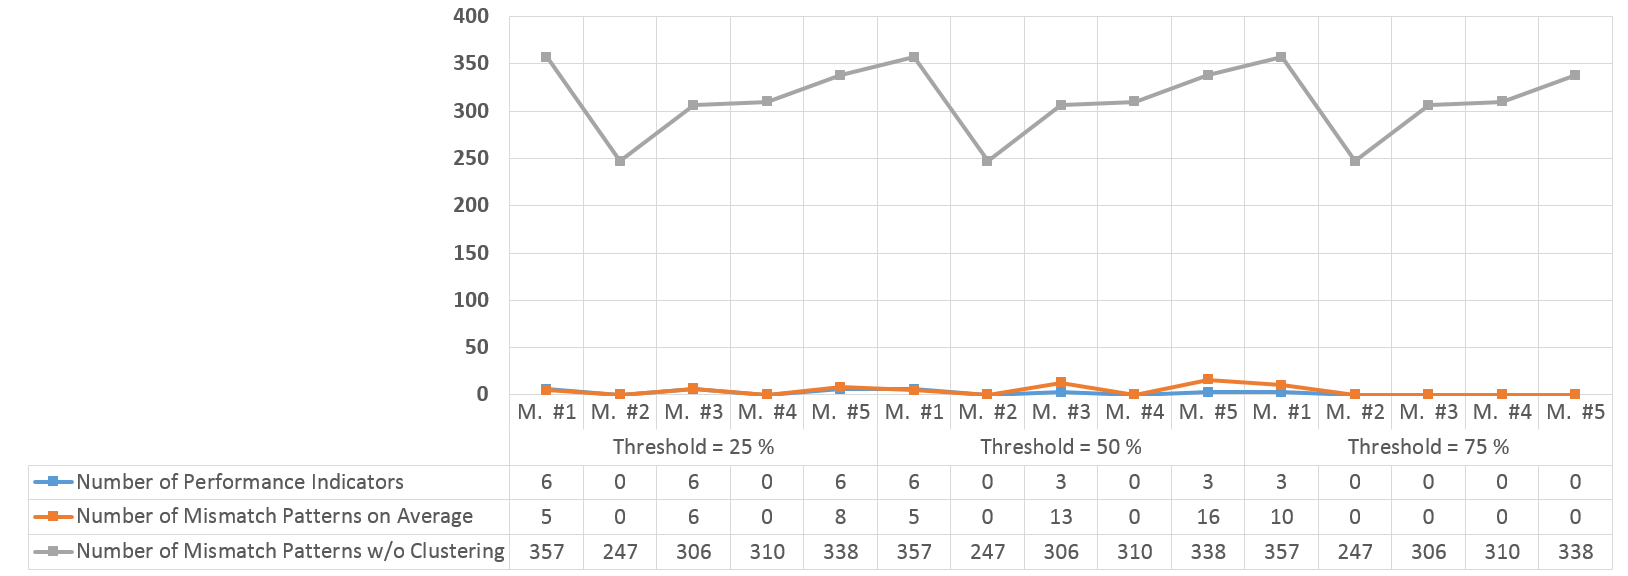
\includegraphics[width=\textwidth]{5_results_discussions/coselog-wabo/recommendation-generation-analysis-k3}
		\caption{Recommendation Generation analysis for Environmental Permit Application Process dataset (3 Clusters)}
	  \label{fig:coselog-wabo-recommendation-generation-analysis}
	\end{figure}
\end{itemize}


\subsection{Discussions}
\label{subsec:discussions}
When the evaluation of the stages for \textit{Loan Application Process} and \textit{Environmental Permit Application Process} datasets are gathered together, the following results can be expressed:

\begin{itemize}
	\item Process mining stage of the proposed methodology can mine the process models with high fitness appropriateness levels.
	\item For the successfully mined models with high fitness values, replay and performance indicator calculation stage works seamlessly as expected. With this step, average and standard deviation time between each activity can be measured for each organization. Number of these metrics are quadratic to the number of activities in each organization's process model and difficult to analyze with a cross comparison.
	\item Internal measure of clusters indicates that the organizations can be clustered according to their performance indicators which yields a collective approach of organizations for their subprocesses. In other words, organizations are divided into clusters which shows that they can be grouped based on how well they are executing.
	\item Mismatch analysis spots the differences between process models in coherence with structural similarity of them. This indicates that the idea of using mismatch patterns to reveal differences between process models is a feasible approach since its results are comparable to the similarity metrics of process models in the literature.
	\item Recommendation generation aims to gather all generated information in this study to help focusing on the potentially important mismatch patterns for performance improvement. When the number of mismatch patterns with and without performance clusterings are checked, it shows that in a small dataset performance clustering lists 3 times less number of differences in \textit{Loan Application Example} dataset. When it is impossible to locate mismatch patterns manually like in \textit{Environmental Permit Application Process}, performance clustering spots 100 times less number of differences. This difference helps user to focus on the differences with a potential performance improvement which is one of the aims in this study.
	\item Although each step of methodology can be counted as successful based on their evaluation metrics, mismatch patterns recommended at the end of methodology can yield important observations as well as being irrelevant and infeasible. Since this decision is based on the business environment of organizations, evaluation of the quality of recommendations for business usefulness requires domain expertise. However, an example recommendation can be presented to provide an insight. In the analysis of \textit{Loan Application Process}, Variant \#3 performs worse 27 \%  on average time and 12 \% on standard deviation time between activities "Calculate Capacity" and "Accept". When the mismatch patterns for these performance indicators are checked the following ones can be mentioned:
		\begin{itemize}
		\item "Check Credit" is a \textit{Refined Activity} of with "Check System (50 \%)"; "Check Paper Archive (42 \%)"; "Send Credit Check Request (32 \%)"; "Process Credit Check Reply (31 \%)" where the corresponding similarity values provided in parentheses.
		\item "Calculate Capacity" is a \textit{Different Moments in Processes} which have different previous activities in clusters. 
		\end{itemize}
	When these example mismatch patterns are checked, removing "Check Credit" activity and putting other activities instead of it might be the cause of performance improvement. With the same approach, putting "Calculate Capacity" on different orders in processes can effect the average and variance of time between activities. These mismatch patterns are also visualized on process model of Variant \#3 and a variant from other cluster in Figure~\ref{fig:loan-recommendation-visualization}. In the process models, refined activities of "Check Credit" and different positions of "Calculate Capacity" are indicated. 
		\begin{figure}
			\centering
			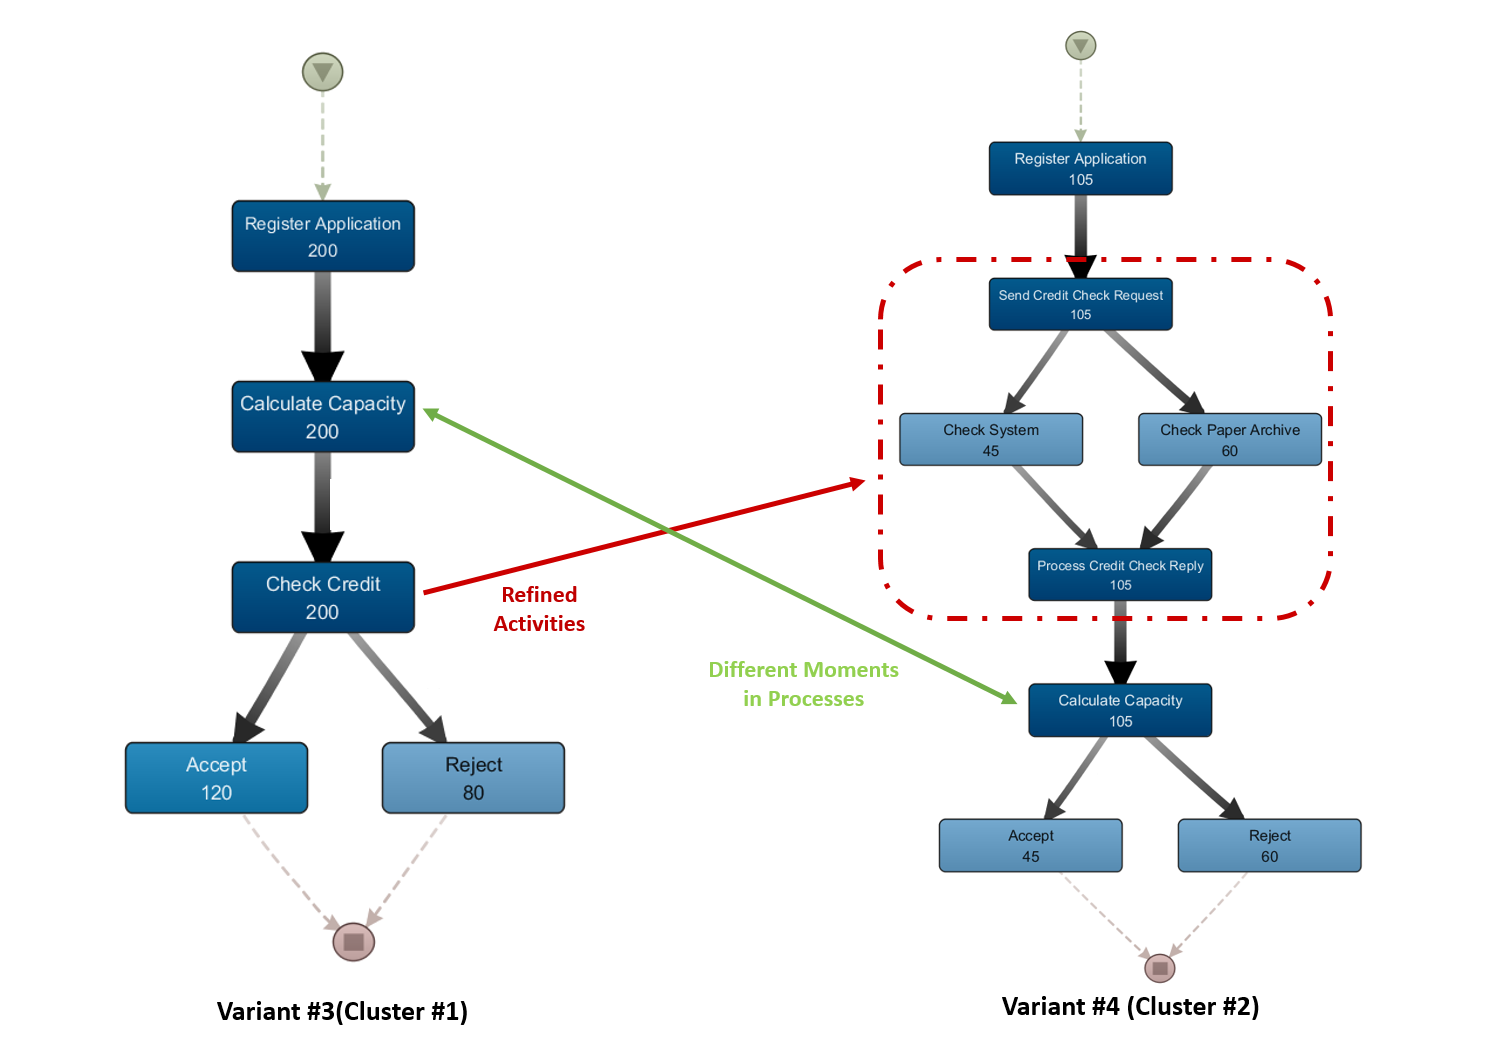
\includegraphics[width=\textwidth]{5_results_discussions/loan-application-process/recommendation-visualization}
			\caption{Visualization of example recommendation for Loan Application Process dataset}
		  \label{fig:loan-recommendation-visualization}
		\end{figure}
\end{itemize} % end of discussions